% !TeX root = main.tex

\hypertarget{confidence-intervals}{%
\section{Confidence Intervals}\label{confidence-intervals}}

\hypertarget{point-estimation}{%
\subsection{Point Estimation}\label{point-estimation}}

\begin{itemize}
\item
  When estimating a population parameter, we may consider the statistic
  of a random sample as an estimate. But we expect some chance error.
\item
  Estimating an unknown parameter by a single number calculated from a
  sample is called a \textbf{point estimation}. The single number
  (statistic) from the sample is called a \textbf{point estimate}.
\item
  Point estimate gives no indication of how reliable the estimate is or
  how large the error is.
\end{itemize}

\begin{example}

From a box of 20 pencils of two colors, black and blue, 10 pencils were
randomly drawn. 6 out of the 10 pencils are black. What proportion of
black pencils are in the box.

\end{example}
\vspace*{6\baselineskip}


\hypertarget{interval-estimation}{%
\subsection{Interval Estimation}\label{interval-estimation}}

\begin{itemize}
\item
  To increase the chance, we estimate an unknown parameter using
  intervals that are obtained by adding chance errors to a point
  estimate.
\item
  Estimating an unknown parameter using an interval of values which
  likely contains the true value of the parameter is called a
  \textbf{interval estimation}. The interval is called an
  \textbf{interval estimate}.
\item
  The reliability of an interval estimate is measured by the probability
  \(1-\alpha\) that the interval estimate will capture the true value of
  the parameter. This probability \(1-\alpha\) is called the
  \href{https://saylordotorg.github.io/text_introductory-statistics/s11-estimation.html}{\textbf{confidence
  level}}.
\item
  The 90\%, 95\% and 99\% levels of confidence are frequently used in
  statistical study. The 95\% level of confidence is usually the
  standard choice of confidence level for scientific polls published in
  the media and online.
\end{itemize}

\begin{example}

Recall that the \textbf{standard error} of a statistic, denoted by SE,
is the standard deviation of the sampling distribution.

A randomly selected 100 students at a college have an average GPA 3.0.
How likely does the interval
\([3.0-2\cdot\text{SE}, 3.0+2\cdot\text{SE}]\) contain the average GPA
\(\mu\) of that college?

\end{example}
\vspace*{6\baselineskip}


\hypertarget{confidence-interval}{%
\subsection{Confidence Interval}\label{confidence-interval}}

\begin{itemize}
\item
  When the sampling distribution of a statistic is approximately
  symmetric, we take interval estimates in the following form
  \([\text{Statistic}- \text{E}, \text{Statistic}+ \text{E}],\) where
  the value \(\text{E}\) is called the \textbf{marginal error} or
  \textbf{margin of error}.
\item
  Given a confidence level \(100(1-\alpha)\%\), the marginal error
  \(\text{E}\) is the value such that \(100(1-\alpha)\%\) of the
  intervals \([\text{Statistic}- \text{E}, \text{Statistic}+ \text{E}]\)
  contains the true parameter \(\mu_\text{par}\). Equivalently, the
  marginal error \(\text{E}\) is the value such that \(100(1-\alpha)\%\)
  of statistics are in the interval
  \([\mu_\text{par}- \text{E}, \mu_\text{par}+ \text{E}]\).
\item
  Denote by \(X\) the random variable for the sample statistic. Then
  \(\text{E}\) is determined the following probability equation
  \[P(\mu_\text{par}-\text{E}< X < \mu_\text{par}+\text{E})=1-\alpha.\]

  If the distribution of \(X\) is symmetric, then the marginal error
  \(E\) is the value such that
  \[P(X-\mu_\text{par}<\text{E})=1-\alpha/2.\]
\item
  Because the parameter \(\mu_\text{par}\) is unknown. If we standardize
  the random variable \(X\) by \(Z=\frac{X-\mu_\text{par}}{\text{SE}}\),
  we get
  \[\textstyle P\left(-\frac{\text{E}}{\text{SE}}<Z<\frac{\text{E}}{\text{SE}}\right)=1-\alpha,\]
  where the random variable \(Z\) has a mean \(0\) and standard
  deviation \(1\).
\item
  The above probability equation suggests the following formula
  \[\textstyle \text{Marginal Error}=\text{Critical value}\cdot \text{Standard Error},\]
  where the \textbf{critical value} is
  \href{https://saylordotorg.github.io/text_introductory-statistics/s11-01-large-sample-estimation-of-a-p.html}{the
  value \(z_{\alpha/2}\) so that
  \(P(-z_{\alpha/2}<Z<z_{\alpha/2})=1-\alpha\)}.
\item
  Let \(X\) be a point estimate, we call the interval
  \([X-z_{\alpha/2}\text{SE}, X+z_{\alpha/2}\text{SE}]\) a
  \textbf{confidence interval} at the \(100(1-\alpha)\%\) level of
  confidence.
\end{itemize}

\textbf{A Visualization of Confidence Intervals for Mean}

\url{https://rpsychologist.com/d3/CI/}

\hypertarget{confidence-intervals-for-mean-with-known-population-sd}{%
\subsection{Confidence Intervals for Mean with Known Population
SD}\label{confidence-intervals-for-mean-with-known-population-sd}}

\begin{itemize}
\item
  Suppose the population standard deviation \(\sigma\) is given. By the
  central limit theorem, if \(n>30\) or the population distribution is
  approximately normal, then the sampling distribution is approximately
  normal with the standard error \(\sigma/\sqrt{n}\).

  At the confidence level \(1-\alpha\), the marginal error for a
  population mean is \(E=z_{\alpha/2}\dfrac{\sigma}{\sqrt{n}}\) and the
  confidence interval is
  \[\left[\bar{x}-z_{\alpha/2}\frac{\sigma}{\sqrt{n}}, \bar{x}+z_{\alpha/2}\frac{\sigma}{\sqrt{n}}\right],\]
  where
  \href{https://saylordotorg.github.io/text_introductory-statistics/s11-01-large-sample-estimation-of-a-p.html}{the
  \textbf{critical value} \(z_{\alpha/2}\) satisfies that
  \(P(Z<z_{\alpha/2})=1-\alpha/2\)} for the standard normal variable
  \(Z\).
\item
  In Excel,\\
  \(z_{\alpha/2}\)=\texttt{NORM.S.INV((1+confidence\ level)/2)}.
\item
  The marginal error \(E=z_{\alpha/2}\frac{\sigma}{\sqrt{n}}\) can also
  be obtained by the Excel function\\
  \texttt{CONFIDENCE.NORM(1-confidence level, $\sigma$, $n$)}.
\end{itemize}

\begin{example}

A sample of size 15 drawn from a normally distributed population with
the standard deviation 6. Find the critical value \(z_{\alpha/2}\)
needed in construction of a confidence interval:

\begin{enumerate}
\item
  when the level of confidence is 90\%;
\item
  when the level of confidence is 98\%.
\end{enumerate}

\end{example}


\begin{example}

A random sample of 50 students from a college gives a mean GPA 2.51.
Suppose the standard deviation of GPAs of all students at the college is
0.43. Construct a 99\% confidence interval for the mean GPA of all
students at the college.

\end{example}
\vspace*{6\baselineskip}


\hypertarget{students-t-distribution}{%
\subsection{\texorpdfstring{Student's
\(t\)-Distribution}{Student's t-Distribution}}\label{students-t-distribution}}

\begin{itemize}
\item
  When the population standard deviation is unknown, we may replace
  \(\sigma\) by the sample standard deviation \(s\) and use
  \(s/\sqrt{n}\) as an estimate to the standard error for the sampling
  distribution of the sample mean.
\item
  When we use the estimated standard error \(s / \sqrt{n}\) to build a
  confidence interval, the normal distribution may NOT be
  appropriate for calculating the critical value. Because the \(t\)-statistic
  \(t=\dfrac{\bar{x}-\mu}{s / \sqrt{n}}\) is not normal in general.
\item
  The random variable \(t=\dfrac{\bar{x}-\mu}{s / \sqrt{n}}\) has approximately a
  \textbf{\href{https://en.wikipedia.org/wiki/Student\%27s_t-distribution}{Student's
  \(t\)-distribution} with the degree of freedom \(n-1\)} 
  if the random variable \(X\) is approximately normal.
\item When the random variable $X$ is not approximately normal but not highly skewed, 
people usually assume that the \(t\)-statistic is normal if the sample size \(n\) is large enough, say, 
\(n\ge 30\).
\end{itemize}

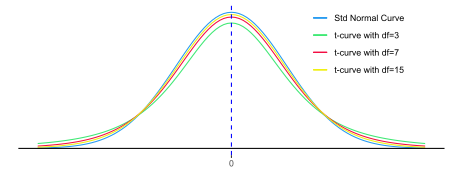
\includegraphics[width=\textwidth]{Figures/t-curves}

\begin{itemize}
\item
  The \(t\)-distributions form a family of curves, called
  \textbf{\(t\)-curves}, parameterized by the
  degrees of freedom.
\item
  The \(t\)-distribution has the following important properties.

  \begin{itemize}
  \item
    Similar to the standard normal curve, it is symmetric about
    0 and the total area under a \(t\)-curve is
    1.
  \item
    The \(t\)-distribution has slightly more variation
    (i.e.~\(t\)-curves are slightly ``fatter'') than the
    standard normal distribution.
  \item
    When the degree of freedom increases, the
    \(t\)-distribution becomes closer to the standard normal
    distribution.
  \end{itemize}
\end{itemize}

\hypertarget{confidence-intervals-for-a-mean-with-unknown-population-sd}{%
\subsection{\texorpdfstring{Confidence Intervals for a Mean with
\textbf{Unknown} Population
SD}{Confidence Intervals for a Mean with Unknown Population SD}}\label{confidence-intervals-for-a-mean-with-unknown-population-sd}}

\begin{itemize}
\item
  Suppose the population is approximately normally distributed or not highly skewed with large sample size.
  At the confidence level \(1-\alpha\), the margin of error is
  \(E=t_{\alpha/2}\frac{s}{\sqrt{n}},\) and the confidence interval for
  a population mean \(\mu\) is
  \[\left[\bar{x}-t_{\alpha/2}\frac{s}{\sqrt{n}}, \bar{x}+t_{\alpha/2}\frac{s}{\sqrt{n}}\right],\]
  where \(t_{\alpha/2}\) is the critical value such that
  \(P(T<t_{\alpha/2})=1-\alpha/2\) for a Student \(t\)-distribution with
  degree of freedom \(n-1\).
\item
  In Excel, the critical value \(t_{\alpha/2}\) can be calculated by\\
  \texttt{T.INV((1+confidence\ level)/2,\ n-1)} or\\
  \texttt{T.INV.2T(1-confidence\ level,\ n-1)},\\ where \(n\) is the
  sample size.
\item
  The marginal error \(E=t_{\alpha/2}\frac{s}{\sqrt{n}}\) can also be
  obtained by the Excel function\\
  \texttt{CONFIDENCE.T(1-confidence\ level,\ s,\ n)}.
\end{itemize}

\begin{example}

A sample of size 15 drawn from a normally distributed population. Find
the critical value \(t_{\alpha/2}\) needed in construction of a
confidence interval:

\begin{enumerate}
\item
  when the level of confidence is 99\%;
\item
  when the level of confidence is 95\%.
\end{enumerate}

\end{example}
\vspace*{3\baselineskip}

\begin{example}

A sample of size 16 is randomly drawn from a normally distributed
population. The sample has a mean 79 and standard deviation 7. Construct
a confidence interval for that population mean at the 90\% level of
confidence.

\end{example}
\vspace*{7\baselineskip}

\begin{example}

The data blow shows numbers of hours worked from 40 randomly selected
employees from several grocery stores in the county.

30, 26, 33, 26, 26, 33, 31, 31, 21, 37, 27, 20, 34, 35, 30, 24, 38, 34, 39, 31,\\
22, 30, 23, 23, 31, 44, 31, 33, 33, 26, 27, 28, 25, 35, 23, 32, 29, 31, 25, 27

Construct 99\% confidence interval for the mean worked time.

\end{example}
\vspace*{10\baselineskip}

\hypertarget{choose-between-normal-distribution-and-t-distribution}{%
\subsection{\texorpdfstring{Choose Between Normal Distribution and
\(t\)-Distribution}{Choose Between Normal Distribution and t-Distribution}}\label{choose-between-normal-distribution-and-t-distribution}}

\begin{itemize}
\item
  Population is approximately normally distributed.

  \begin{itemize}
  \item
    the population standard deviation \(\sigma\) is known:
    use the normal distribution.
  \item
    the population standard deviation \(\sigma\) is
    \emph{unknown}: use the
    \(t\)-\emph{distribution}.
  \end{itemize}
\item
  Population distribution unknown but \textbf{not highly skewed}. If the \textbf{sample size is large}
  enough, i.e.~\(n>30\), then

  \begin{itemize}
  \item
    the population standard deviation \(\sigma\) is known:
    use normal distribution.
  \item
    the population standard deviation \(\sigma\) is
    \emph{unknown}: either one can be used but the
    \(t\)-\emph{distribution} is more accurate.
  \end{itemize}
\item
  \textbf{Warning:} When the population distribution is unknown and the
  sample size is small, neither the \(t\)-distribution nor the
  normal distribution is reliable.
\item
  For small samples, there is method called
  ``\href{http://www.sthda.com/english/wiki/normality-test-in-r\#normality-test}{The
  Shapiro--Wilk test}'' which can be used to determine if we may assume
  the sampling distribution is approximately normal.
\item
  Even when \(n>30\), a visual inspection (using histogram for example)
  of the normality is necessary.
\end{itemize}

\hypertarget{practice}{%
\subsection{Practice}\label{practice}}

\begin{exercise}

Decide whether the following statements are true or false. Explain your
reasoning.

\begin{itemize}
\item
  The statement, ``the 95\% confidence interval for the population mean
  is (350, 400)'' means that 95\% of the population values are between
  350 and 400.
\item
  For a given standard error, lower confidence levels produce wider
  confidence intervals.
\item
  If you increase sample size, the width of confidence intervals will
  increase.
\item
  If you take large random samples over and over again from the same
  population, and make 95\% confidence intervals for the population
  average, about 95\% of the intervals should contain the population
  average.
\end{itemize}
\end{exercise}

\begin{exercise}

A sample of 34 watermelons' have a mean weight of 64 ounces. Assume the
population standard deviation is 12.7 ounces. Based on this, what is the
maximal margin of error associated with a 90\% confidence interval for
the true population mean watermelon weight.

\end{exercise}
\vspace*{8\baselineskip}

\begin{exercise}

If a school district takes a random sample of 70 Math SAT scores and
finds that the average is 426, and knowing that the population standard
deviation of Math SAT scores is intended to be 100. Find a 99\%
confidence interval for the mean math SAT score for this district.

\end{exercise}
\vspace*{8\baselineskip}

\begin{exercise}

In a survey, 32 people were asked how much they spent on their child's
last birthday gift. The results were roughly bell-shaped with a mean of
\$39 and standard deviation of \$7. Find the margin of error at a 80\%
confidence level.

\end{exercise}
\vspace*{8\baselineskip}

\begin{exercise}

A statistics student is curious about drinking habits of students at his
college. He wants to estimate the mean number of alcoholic drinks
consumed each week by students at his college. He plans to use a 90\%
confidence interval. He surveys a random sample of 71 students. The
sample mean is 3.93 alcoholic drinks per week. The sample standard
deviation is 3.78 drinks.

\end{exercise}
\vspace*{8\baselineskip}

\begin{exercise}

Four hundred randomly selected working adults in a certain state,
including those who worked at home, were asked the distance from their
home to their workplace. The average distance was 8.84 miles with
standard deviation 2.70 miles.

Construct a 98\% confidence interval for the mean distance from home to
work for all residents of this state.

\end{exercise}
\vspace*{8\baselineskip}

\begin{exercise}

City planners wish to estimate the mean lifetime of the most commonly
planted trees in urban settings. A sample of 16 recently felled trees
yielded mean age 32.7 years with standard deviation 3.1 years. Assuming
the lifetimes of all such trees are normally distributed, construct a
99.8\% confidence interval for the mean lifetime of all such trees.

\end{exercise}
\vspace*{8\baselineskip}

\begin{exercise}

Assuming the the population is normally distributed, find the 90\% confidence interval for the population mean using the following sample.

45.8, 56.8, 65, 67.5, 30.4, 43.9, 59.7, 51.3

\end{exercise}
\vspace*{8\baselineskip}

\hypertarget{lab-confidence-intervals}{%
\subsection{Lab: Confidence Intervals}\label{lab-confidence-intervals}}

\subsubsection{Excel Functions for
\(t\)-Distributions}

Suppose a Student's \(t\)-distribution has the degree of freedom
\(\text{df}=n-1\).

\begin{itemize}
\item
  Find a probability for a given \(t\)-value.

  \begin{itemize}
  \item
    The area of the left tail of the \(t\)-value may be calculated by
    the function \texttt{T.DIST(t,df,true)}.
  \item
    The area of the right tail of the \(t\)-value may be calculated by
    the function \texttt{T.DIST.RT(t,df)}.
  \item
    The area of two tails of the \(t\)-value (here \(t\)> 0)
    may be calculated by function \texttt{T.DIST.2T(t,df)}.
  \end{itemize}
\item
  Find the critical value for a given probability \(p\).

  \begin{itemize}
  \item
    When the area of the left tail is given, the function
    \texttt{T.INV(p,df)} may be used.
  \item
    When the area of both tails is given, the function\\
    \texttt{T.INV.2T(p,df)}\\
    may be used. This function is good for
    construction confidence interval.
  \end{itemize}
\end{itemize}

\hypertarget{excel-functions-for-marginal-errors}{%
\subsubsection{Excel Functions for Marginal
Errors}\label{excel-functions-for-marginal-errors}}

\begin{itemize}
\item
  If the population standard deviation \(\sigma\) is given and the
  sampling distribution is approximately normal, the marginal error can be obtained by the Excel function\\
  \begin{fullwidth}
    \colorbox{white}{
      \texttt{CONFIDENCE.NORM(1-confidence\ level,\ population\ SD,\ sample\ size)}
    }
  \end{fullwidth}
\item
  If the population standard deviation \(\sigma\) is NOT given and the
  sampling distribution is approximately normal, the marginal error can
  be obtained by the Excel function, the marginal error can be obtained by the Excel function

  \begin{fullwidth}
    \colorbox{white}{
      \texttt{CONFIDENCE.T(1-confidence\ level,\ sample\ SD,\ sample\ size)}
    }
  \end{fullwidth}
\end{itemize}

\begin{exercise}

A sample of size 28 randomly selected to estimate a population mean with
a confidence interval. The population is approximately normally
distributed.

Find the critical value that corresponds to a confidence level of 80\%.

\end{exercise}
\vspace*{6\baselineskip}

\begin{exercise}

A sample of 22 backpacks' have a mean weight of 77 ounces. Assume the
population standard deviation is 11.3 ounces. Based on this, what is the
maximal margin of error associated with a 95\% confidence interval for
the true population mean backpack weight.

\end{exercise}
\vspace*{6\baselineskip}

\begin{exercise}

In a survey, 21 people were asked how much they spent on their child's
last birthday gift. The results were roughly bell-shaped with a mean of
\$34 and standard deviation of \$6. Find the margin of error at a 98\%
confidence level.

\end{exercise}
\vspace*{6\baselineskip}

\begin{exercise}

Assuming the the population is normally distributed. Find the 99.5\%
confidence interval for the population mean using the following sample.

97.8, 90.4, 76.9, 88.6, 97.1, 87.8, 88, 69.9, 75.3, 81.6

\end{exercise}
\vspace*{6\baselineskip}

